\head{Октябрь}{Листок 9. Комбинаторика -- 2. Уровень 2.}

\section{И снова числа сочетаний.}

Итак,

\begin{enumerate}[label=\asbuk*), ref=\asbuk*]
    \item $C^0_n + C^1_n + C^2_n + ... + C^n_n = 2^n$ -- количество всех подмножеств $n$--элементного множества.
    \item $C^0_n - C^1_n + C^2_n - ... + (-1)^n C^n_n$ -- доказывает тот факт, что количество подмножеств из четного числа элементов всегда равно количеству подмножеств из нечетного числа элементов.
    \item $(C^0_n)^2 + (C^1_n)^2 + (C^2_n)^2 + ... + n C^n_n = n 2^{n - 1}$ -- количество способов выбрать $n$ элементов из $2n$ -- элементного множества.
    \item \label{ravenstvo4} $C^1_n + 2C^2_n + 3C^3_n + ... + nC^n_n = n2^{n-1}$ -- количество единиц при выписывании всевозможных последовательностей длины $n$ из нулей и единиц.
    \item \label{ravenstvo5}  $C^k_n = \dfrac{n}{k}C^{k - 1}_{k - 1}$ -- просто полезная формула.
\end{enumerate}

Равенство \ref{ravenstvo4}) мы доказывали, не опираясь на задачу о последовательностях. Напомним, как. 
\\ Мы знаем, что $C^k_n = C^{n - k}_n$, поэтому левую часть требуемого равенства можно переписать как 
\\ $n C^0_n + (n - 1) C^1_n + (n - 2 + 2) C^2_n + ... + C^{n-1}_n + 0 \cdot C^n_n$. Сложим полученное выражение с уже имеющимся: $n C^0_n + (n - 1 + 1) C^1_n + (n - 2 + 2) C^2_n + ... + (1 + n - 1) C^{n-1}_n + (0 + n) C^n_n = n (C^0_n + C^1_n + C^2_n + ... + C^n_n) = n 2^n$.
Тем самым мы сосчитали удвоенную требуемую сумму. Следовательно, сама сумма равна $n 2^{n–1}$.

\par

Отметим, что использованный нами приём очень распространен. Например, аналогично можно вывести формулу для суммы первых $n$ натуральных чисел.
\\
S = 1 + 2 + 3 + ... + $n$ = $n$ + ($n$ $-$ 1) + ... 3 + 2 + 1. Отсюда 2S = (1 + n) + (2 + n $-$ 1) + (3 + n $-$ 2) + ... + ($n$ $-$ 1 + 2) + ($n$ + 1) = $n$ ($n$ + 1). Для удобства будем называть разобранный способ доказательства \textit{методом сложения}.

\begin{dfn}
    Последовательность чисел ${a_n}$ называется \textit{арифметической прогрессией}, если разница между любыми двумя соседними членами одинакова, т.е. $\forall k \in a_{k+1} - a_k = d$ (или $a_{k + 1} = a{k} + d$). Эта разница называется \textit{разностью} или \textit{приращением} арифметической прогрессии. В частности натуральный ряд – это арифметическая прогрессия с разностью 1.
\end{dfn}

\begin{thm}
    Пользуясь методом сложения, выведите формулу для суммы первых $n$ членов арифметической прогрессии (первый член и разность считаются заданными).
\end{thm}

\begin{thm}
    Аналогичным способом вычислите сумму $C^0_n + 2 C^1_n + 3 C^2_n + 4 C^3_n + ... + (n + 1) C^n_n$.
\end{thm}

\begin{thm}
    Вычислите сумму $C^2_n + 2 C^3_n + ... + (n - 1) C^n_n$.
\end{thm}

\begin{thm}
    Вычислите сумму $C^0_n + 3 C^1_n + 5 C^2_n + 7 C^3_n + ... + (2n + 1) C^n_n$.
\end{thm}

\begin{thm}
    Вычислите сумму $3 C^1_n + 7 C^2_n + 11 C^3_n ... + (4n - 1) C^n_n$.
\end{thm}

\begin{thm}
    Вычислите сумму $C^1_n + 2 C^2_n + 3 C^3_n ... + (-1)^{n - 1} n C^n_n$.
\end{thm}

\begin{prf}
    Воспользуемся равенством $C^k_n = C^k_{n - 1} + C^{k - 1}_{n - 1}$. . Искомая сумма равна $S = C^1_{n - 1} + C^0_{n - 1} - 2 (C^2_{n - 1} + C^1_{n - 1}) + 3 (C^3_{n - 1} + C^2_{n - 1}) + ... + (-1)^{n - 1} n C^{n - 1}_{n - 1} = C^0_{n - 1} - C^1_{n - 1} + 2 C^2_{n - 1} - C^3_{n - 1} + ... + (-1)^{n - 1} C^{n - 1}_{n - 1} = 0$ при $n > 1$. 
    \\ Очевидно, что при $n = 1$ эта сумма равна 1.
\end{prf}

\textit{\underline{Замечание.}} Отметим, что для нечётных $n$ равенство легко доказывается методом сложения. 
\\ Всего можно отметить три основных способа доказательства утверждений комбинаторики, в частности равенств о биноминальных коэффициентах. Первый основан на том, что $C^k_n$ -- количество $k$ -- элементных подмножеств $n$ -- элементного множества, второй – на том, что $C^k_n$ -- коэффициент при $x^k$ в разложении $(1 + x)^n$, третий использует свойства треугольника Паскаля, в частности, что $C^k_n$ -- число путей из верхней клетки в $k$ -- ю клетку $n$ -- ой строки. Третьим способом очень элегантно доказывается равенство в) про сумму квадратов. Равенства а) и б) легко получаются, применяя второй способ. Поговорим о первом способе. Напомним доказательство равенства $C^k_n = C^k_{n - 1} + C^{k - 1}_{n - 1}$. Мы среди имеющихся $n$ предметов фиксировали один. После чего рассматривали отдельно выборки включающие этот предмет -- их $C^k_{n - 1}$ и не включавшие его -- их $C^{k - 1}_{n - 1}$.
\\ Складывая, получаем требуемое равенство.

\begin{thm}
    Докажите, что $(C^0_n)^2 + (C^1_n)^2 + (C^2_n)^2 + ... + (C^n_n)^2 = C^n_{2n}$ всеми тремя способами.\footnotemark
\end{thm}\footnotetext{При доказательстве утверждений с помощью бинома Ньютона мы пользуемся фактом, что многочлены тождественно равны тогда и только тогда, когда равны их коэффициенты при соответствующих степенях.}

\begin{thm}
    Докажите, что $(C^0_{2n})^2 + (C^1_{2n})^2 + (C^2_{2n})^2 + ... + (C^{2n}_{2n})^2 = (-1)^n C^n_{2n}$  (знаки в сумме чередуются).
\end{thm}

Разберём ещё два примера.

\begin{thm}
    Докажите, что $C^1_n + 6C^2_n + 6C^3_n = n^3$.
\end{thm}

\begin{prf}
    Заметим, что $n^3$ – это количество способов, какими можно выбрать три предмета из $n$, если
предметы разрешается повторять (например, покрасить три полоски флага, если имеется $n$ возможных цветов – часто такую выборку называют \textit{размещением с повторением}, а само количество способов – \textit{число размещений с повторениями}). Попробуем \textit{увидеть} это же в левой части требуемого равенства. Для этого разобьем все возможные выборки на три непересекающихся типа: 
\\ \underline{первый тип}: все три предмета одинаковы, понятно, что таких способов ровно столько же, сколько и всего различных предметов, т.е. $n = С^1_n$;
\\ \underline{второй тип}: имеется два одинаковых предмета. Выбрать два предмета можно $C^2_n$ способами и ещё 6 способов разместить их на три места. 
\par И, наконец, 
\\ \underline{третий тип}: все три предмета различны. Выбрать три предмета можно $С^3_n$ способами и ещё 6 вариантов их размещения на три места. 
\par Тем самым, искомое равенство доказано.
\end{prf}

\begin{ex}
    Сосчитайте, сколькими способами можно раскрасить флажок из $k$ полосок 
    \\ а) в два цвета (оба цвета обязаны присутствовать); б) в три цвета; в$^*$) в $р (р < k)$ цветов.
\end{ex}

\begin{thm}
    Докажите, что $1 + 7C^1_n + 12C^2_n + 6C^3_n = (n + 1)^3$.
\end{thm}

\begin{prf}
    Будем рассматривать $n + 1$ предмет, среди которых один особенный. По аналогии с предыдущей задачей можно рассмотреть размещения с повторениями, в которые входит особенный предмет и в которые не входит. Число размещений без особенного предмета равно $n^3 = С^1_n + 6С^2_n + 6С^3_n$. Сосчитаем теперь число размещений, в которые обязательно входит особенный предмет. 
    \\Первый случай: все три предмета –
особенные, такой вариант только один.
\\ Второй случай: один или два предмета особенные, а остальные –
какого-то одного другого типа, тогда количество способов выбрать этот другой тип равно $C^1_n$ и умножаем на
6 = количество способов расположить эти предметы на три места. 
\\ И третий случай: только один предмет
особенный, а два другие различны. Тогда число способов равно $6C^2_n$. 
\par Теперь, складывая полученные
значения, мы получаем требуемое равенство.
\end{prf}

Ранее мы говорили о коэффициентах многочлена, полученного после раскрытия скобок в выражении
$(a + b)^n$. (Заметим, что зная обозначения для биномиальных коэффициентов, можно записать нашу
формулу в более коротком универсальном виде: $(а + b)^n = \underset{k = 0}{\overset{n}\sum} C^k_n a^k b^{n - k}$.) Применяя формулу бинома
Ньютона, можно раскладывать и более сложные выражения.

\par

Например, $(a + b + c)^4 = ((a + b) + c)^4 = \underset{k = 0}{\overset{4}{\sum}} C^k_4 (a + b)^k c^{4 - k} = ...$, пользуясь далее формулами уже для выражений $(a + b)^n$. Однако, такой способ слишком сложен уже для небольших степеней, а если степени выше 4? Кроме того с помощью такого способа сложно сразу указать коэффициент при каком-нибудь одночлене (сразу угадывается, пожалуй, только коэффициенты при самых старших степенях). Попробуем
найти другой способ.

\par

При доказательстве формулы для $(a + b)^n$ мы пользовались тем фактом, что коэффициент при одночлене $a^k b^{n – k}$ равен количеству способов выбрать $k$ скобок (или же $n – k$) из $n$. Попытаемся осуществить ту же идею для трёх слагаемых. Понятно, что количество слагаемых вида $a^{k_1} b^{k_2} c^{k_3}$ равно количеству способов, сколькими можно выбрать $k_1$ предметов из имеющихся $n$, а из оставшихся $n – k_1$
предметов ещё $k_2$ предметов.

\begin{thm} \label{9.0 thm 9.0}
    Имеется $n$ различных предметов и $m$ ящиков. Нужно положить в первый ящик $k_1$ предметов, во второй -- $k_2$, в третий -- $k_3$, ... , в $m$-ый -- $k_m$, если $k_1 + k_2 + k_3 + ... + k_m = n$. Докажите, что число способов это сделать равно $P(k_1, k_2, k_3, ... , k_m) = \dfrac{n!}{k_1!k_2!...k_m!}$. 
\end{thm}

Таким образом, пользуясь задачей \ref{9.0 thm 9.0} мы можем вывести формулу для многочлена, полученного после
раскрытия скобок в выражении $(a + b + c)^n = \sum P(k_1, k_2, k_3) a^{k_1} b^{k_2} c^{k_3} = \sum \dfrac{n!}{k_1!k_2!k_3!} a{^k_1} b{^k_2} c{^k_3}.$

\begin{ques}
    Верно ли, что все коэффициенты в этом разложении различны?
\end{ques}

\begin{thm}
    Вычислите сумму:
    \par а) $C^0_5 + 2^1 \cdot C^1_5 + 2^2 \cdot C^2_5 + 2^3 \cdot C^3_5 + 2^4 \cdot C^4_5 + 2^5 \cdot C^5_5$
    \par  б)  $3^0 \cdot C^0_n + 3^1 \cdot C^1_n + 3^2 \cdot C^2_n + ... + 3^{n - 1} \cdot C^{n - 1}_n + 3^n \cdot C^n_n$
\end{thm}

\begin{thm}
    Докажите, что $C^{k + 1}_n = \dfrac{n - k}{k + 1} C^k_n$
\end{thm}

\begin{thm} $^*$
    Докажите, что $C^1_n + 14C^2_n + 36C^3_n + 24C^4_n = n^4$.
\end{thm}

\begin{thm} $^*$
    Докажите, что $C^1_n + 14C^2_n + 36C^3_n + 24C^4_n = n^4$
\end{thm}

\begin{thm} $^*$
    Докажите, что $1 + 14C^1_n + 36C^2_n + 24C^3_n + = (n + 1)^4 - n^4$.
\end{thm}

\begin{thm} $^*$ \label{9.0 thm1}
    Докажите, что $\underset{i = 0}{\overset{k}\sum} C^i_n C^{k - i}_m =  C^0_n C^k_m + C^1_n C^{k - 1}_m + ... + C^k_n C^0_m = C^k_{n + m} (k \leq m, k \leq n)$.
\end{thm}

\begin{thm} $^*$ \label{9.0 thm2}
    Докажите, что $C^{k - 1}_{n - 1} + C^{k - 1}_{n - 2} + ... + C^{k - 1}_{k - 1} = C^k_n (k \leq n)$.
\end{thm}

\textit{\underline{Замечание}}. Решите задачи \ref{9.0 thm1} и \ref{9.0 thm2} двумя – тремя способами.

\begin{thm} $^{**}$
    Докажите, что $(C^1_n)^2 + 2(C^2_n)^2 + 3(C^3_n)^2 + ... n (C^n_n)^2 = \dfrac{(2n - 1)!}{[(n - 1)!]^2}$.
\end{thm}

(\textit{\underline{Указание}}. Воспользуйтесь полезной формулой \ref{ravenstvo5} и тем, что $n (1 + x)^{2n–1} = n(1 + x)^{n–1} (1 + x)^n$, после чего найдите
нужную степень $x$ и сравните коэффициенты.)

\begin{thm} $^{**}$
    Докажите, что $\dfrac{1}{[(n - 1)!]^2} + \dfrac{1}{1!2!} \dfrac{1}{[(n - 2)!]^2} + \dfrac{1}{2!3!} \dfrac{1}{[(n - 3)!]^2} + ... = \dfrac{(2n - 1)!}{[n!(n - 1)!]^2}$.
\end{thm}

(\textit{\underline{Указание}}. Преобразуйте выражения с факториалами к биномиальным коэффициентам).

\begin{thm} $^{**}$
    \textit{(Свойство шестиугольника)} Докажите равенство $C^{k - 1}_{n - 1} \cdot C^{k + 1}_n \cdot C^k_{n + 1} = C^k_{n - 1} \cdot C^{k + 1}_{n + 1} \cdot C^{k - 1}_n$ без использования явных формул для биномиальных коэффициентов. 
\end{thm}

\begin{thm} $^*$
    В  пирамиду выстроены $n$ кубиков $n$ различных цветов. Максим развлекается тем, что аккуратно вынимает снизу пирамиды от 1 до $n$ кубиков и устанавливает их в том же порядке сверху пирамиды, после чего переворачивает пирамиду вверх ногами и повторяет операцию. Сколько различных пирамид может получиться у Максима в процессе этого развлечения?
\end{thm}

\section{Задача для размышления.}

\begin{thm} $^*$
    Имеется бесконечно продолжающаяся вправо и вверх клетчатая доска. В её левом нижнем углу стоит шашка. За один ход с доски снимается одна шашка, а вместо неё выставляется две – одна правее, другая выше исходной (на рисунке сделано четыре хода - та шашка, что снимается, отмечена серым). Можно ли, сделав несколько ходов, добиться того, чтобы в выделенном квадрате $3 \times 3$ не осталось ни одной шашки? % Извините
    
    \begin{tabular}{ |m{.5em}|m{.5em}|m{.5em}|m{.5em} } 
     & & & \\ 
    \hline
     & & & \\
    \hline
     & & & \\
    \hline
    \makecircle{black}{gray} & & & \\
    \hline
    \end{tabular}
        \hfill
            $\rightarrow$
        \hfill
    \begin{tabular}{ |m{.5em}|m{.5em}|m{.5em}|m{.5em} } 
     & & & \\ 
    \hline
     & & & \\
    \hline
    \makecircle{black}{gray} & & & \\
    \hline
     & \makecircle{black}{white} & & \\
    \hline 
    \end{tabular}
        \hfill
            $\rightarrow$
        \hfill
    \begin{tabular}{ |m{.5em}|m{.5em}|m{.5em}|m{.5em} } 
     & & & \\ 
    \hline
    \makecircle{black}{white} & & & \\
    \hline
     & \makecircle{black}{gray} & & \\
    \hline
     & \makecircle{black}{white} & & \\
    \hline
    \end{tabular}
        \hfill
            $\rightarrow$
        \hfill
    \begin{tabular}{ |m{.5em}|m{.5em}|m{.5em}|m{.5em} } 
     & & & \\ 
    \hline
    \makecircle{black}{white} & \makecircle{black}{white} & & \\
    \hline
     & & \makecircle{black}{white} & \\
    \hline
     & \makecircle{black}{gray} & & \\
    \hline
    \end{tabular}
        \hfill
            $\rightarrow$
        \hfill
    \begin{tabular}{ |m{.5em}|m{.5em}|m{.5em}|m{.5em} } 
     & & & \\ 
    \hline
    \makecircle{black}{white} & \makecircle{black}{white} & & \\
    \hline
     & \makecircle{black}{white} & \makecircle{black}{white} & \\
    \hline
     & & \makecircle{black}{white} & \\
    \hline
    \end{tabular}

\end{thm}

\section{Комбинаторая солянка задач.}

\begin{figure}[H]
\begin{minipage}{0.59\linewidth}\setlength{\parindent}{1.5em}
    \begin{thm}
        Из пункта $A$ по сети дорог идёт группа туристов из 27 человек. (см.рис.) На каждом перекрёстке, начиная с $A$, туристы делятся пополам – одна половина идёт по направлению $l$, а другая половина – по направлению $m$. Сколько человек придёт в пункты $B$, $C$, $D$, ... , $I$ соответственно?
    \end{thm}
    \begin{thm}
        Докажите, что $\dfrac{(2n)!}{n!n!}$ делится на $n + 1$.
    \end{thm}
    \begin{thm}
        В ряд стоят 50 стульев. Сколькими способами можно убрать 20 из них, если нельзя убирать никакие два стула, стоящих рядом?
    \end{thm}
\end{minipage}
\hfill
\begin{minipage}{0.4\linewidth}
    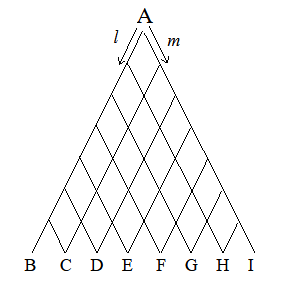
\includegraphics[width=0.95\columnwidth]{img/9.0 triangle.png}
\end{minipage}
\end{figure} 

\begin{thm}
    Фабрика окрашивает кубики в 6 цветов (каждую грань в свой цвет, набор цветов фиксирован). Сколько разновидностей кубиков можно изготовить?
\end{thm}

\begin{thm}
    На окружности даны 10 точек. Сколькими способами можно провести пять непересекающихся отрезков с концами в заданных точках?
\end{thm}

\begin{thm}
    Имеется прямоугольная доска $30 \times 40$. Найдите число прямоугольников, составленных из клеток этой доски.
\end{thm}

\begin{thm}
    У Кости есть $n$ друзей, и каждый день он приглашает некоторых из них в гости так, чтобы компания ни разу не повторялась (в какой-то день он может не пригласить никого). Сколько дней он сможет так делать?
\end{thm}

{\setlength{\intextsep}{2pt}
\begin{figure}[h]
\begin{minipage}{0.55\linewidth}\setlength{\parindent}{1.5em}
    \begin{thm}
    Сколькими способами можно добраться из пункта А
в пункт В по линиям сетки без самопересечений?
    \end{thm}
\end{minipage}
\hfill
\begin{minipage}{0.35\linewidth}\setlength{\parindent}{1.5em}
    A \begin{tabular}{ |m{.1em}|m{.1em}|m{.1em}|m{.1em}|m{.1em}|m{.1em}|m{.1em}|m{.1em}|m{.1em}|c| } 
    \hline
     & & & & & & & & & \\ 
    \hline
    \end{tabular} B
\end{minipage}
\end{figure}}

\begin{thm}
    Сколькими способами можно из последовательности 1, 2, ..., 2$n$ выбрать три числа, образующих арифметическую прогрессию?
\end{thm}

\begin{thm}
    У Вани есть кучка из 2012 морковок. Каждую минуту он произвольным образом делит одну из имеющихся у него кучек на две до тех пор, пока не получит 2012 кучек по одной морковке. При каждом делении Ваня записывает произведение числа морковок в получившихся двух кучках. Чему в результате равна сумма этих произведений?
\end{thm}

\begin{thm}
    Найдите количество клетчатых прямоугольников шахматной доски, содержащих клетку с4.
\end{thm}

\begin{thm}
    Сколько наборов целых чисел удовлетворяют условию:
    \par
    а) $0 < a_1 < a_2 < ... < a_n < n$; \hfill б) $0 \leq a_1 \leq a_2 \leq ... \leq a_n \leq n$? 
\end{thm}

\begin{thm}
    Сколько наборов целых неотрицательных чисел удовлетворяют условию:
    \par
    а) $a_1 + a_2 + ... + a_n = n$; \hfill б) $a_1 + a_2 + ... + a_n \leq n$? 
\end{thm}